\documentclass[crop=false,fleqn]{standalone}
\usepackage{../../../globle-preamble}

\begin{document}
    \textbf{Find the domain and range of the funtion $g$ and sketch graph of $g$.}

    $$
    g(x) = \frac{x^2-16}{x-4}\quad, \quad x \ne 4
    $$

    \vspace{1em}
    Domain of $g(x)$ = $\mathbb{R}$

    Rang of $g(x)$ = $\mathbb{R}$
    \vspace{1em}

    \begin{center}
        \begin{tabular}{ |c|c|c|c|c|c|c|c| } 
            \hline
            $x$ & -1 & 0 & 1 & 2 & 3 & 5 & 6 \\ 
            \hline
            $g(x)$ & 3 & 4 & 5 & 6 & 7 & 9 & 10 \\
            \hline
        \end{tabular}
    \end{center}

    \begin{center}
        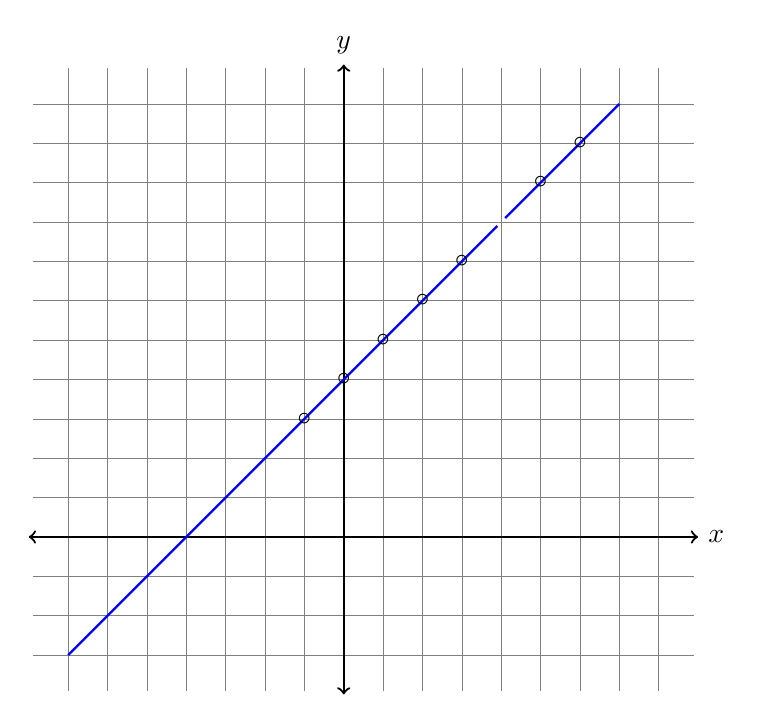
\begin{tikzpicture}[scale=0.5]
            \draw[step=1,gray,very thin] (-7.9,-3.9) grid (8.9,11.9);
            \draw[<->,thick] (-8, 0) -- (9, 0) node[right] {$x$};
            \draw[<->,thick] (0, -4) -- (0, 12) node[above] {$y$};

            \draw[domain=-7:3.9, smooth, variable=\x, thick, blue] plot ({\x}, {(\x+4)});
            \draw[domain=4.1:7, smooth, variable=\x, thick, blue] plot ({\x}, {(\x+4)});

            \foreach \Point in {(-1,3), (0,4), (1,5), (2,6), (3,7), (5,9), (6, 10)}{
                \node at \Point {$\circ$};
            }
        \end{tikzpicture}
    \end{center}
\end{document}
